\documentclass[compress]{beamer}

\usetheme{CambridgeUS}
\usecolortheme{rose}

\usepackage{amsmath,amsfonts,amssymb}
\usepackage{caption}
\usepackage{enumerate}
\usepackage{graphicx}
\usepackage{floatrow}
\usepackage{hyperref}
\hypersetup{
    colorlinks=true,
    linkcolor=blue,
    filecolor=magenta,
    urlcolor=cyan,
}
% \captionsetup[table]{labelformat=empty}
\newcommand{\expect}[1]{\mathbb{E} \left[ #1 \right]}
\newcommand{\expects}[2]{\mathbb{E}_{#1} \left[ #2 \right]}


\title{Model-Agnostic Meta-Learning for Fast Adaptation of Deep Networks}
\author[Presentor: Shih-Ming Wang]{Chelsea Finn, Pieter Abbeel,  Sergey Levine}
\institute[]{Presented by Shih-Ming Wang}
\date{10-30-2019}
\subject{Computer Science}
\graphicspath{{img/}}


\begin{document}

\begin{frame}
    \maketitle
    % \hypertarget{titlePage}{}
\end{frame}

\begin{frame}
    \frametitle{Authors}

    \begin{columns}
        \begin{column}{.3\textwidth}
            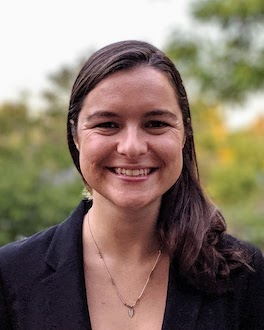
\includegraphics[width=\textwidth,height=.5\textheight]{auth1}
        \end{column}
        \begin{column}{.2\textwidth}
            \tiny
            \textbf{Chelsea Finn} \\
            Assistant Professor \\
            CS, Stanford University \\
        \end{column}
        \begin{column}{.3\textwidth}
            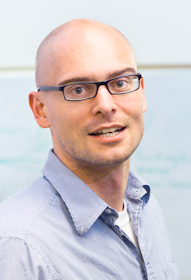
\includegraphics[width=\textwidth,height=.5\textheight]{auth2}
        \end{column}
        \begin{column}{.2\textwidth}
            \tiny
            \textbf{Pieter Abbeel} \\
            Professor \\
            EECS, UC Berkeley \\
        \end{column}
    \end{columns}
    \vfill
    \begin{columns}
        \begin{column}{.3\textwidth}
            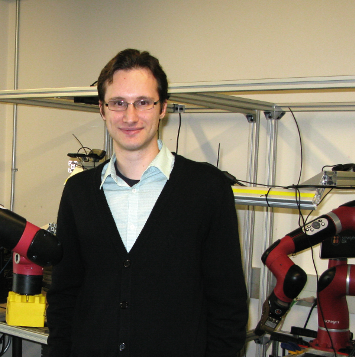
\includegraphics[width=\textwidth,height=.5\textheight]{auth3}
        \end{column}
        \begin{column}{.2\textwidth}
            \tiny
            \textbf{Sergey Levine} \\
            Assistant Professor \\
            EECS, UC Berkeley \\
        \end{column}
        \begin{column}{.3\textwidth}
        \end{column}
        \begin{column}{.2\textwidth}
        \end{column}
    \end{columns}

\end{frame}

\section{Introduction}
\begin{frame}[allowframebreaks]{Introduction}
    \begin{block}{Meta-Learning on Wiki}
        \begin{enumerate}
            \item Traditional machine learning is based on a set of assumptions about the data, its ``inductive bias'', which means a learning algorithm will work well if the bias matches the learning problem.
            \item By using different kinds of meta data, like properties of the learning problem, algorithm properties (like performance measures), or patterns previously derived from the data, it is possible to learn, select, alter or combine different learning algorithms to effectively solve a given learning problem.
        \end{enumerate}
    \end{block}
    \begin{block}{Machine Learning 101}
        \begin{enumerate}
            \item The error of a machine learning algorithm is composed of two terms
                \begin{enumerate}
                    \item bias error: simple model can't capture the true data distribution
                    \item variance error: complex model can capture the true data distribution but requires more data to reduce the possibility of overfit.
                \end{enumerate}
            \item Usually, the model complexity is decided before we see the data, otherwise, we are overfitting the data by our brain
            \item Therefore, meta-learning is a technique that use meta-data to dynamically change the model's inductive bias to a strong bias (low variance) that capture the true data distribution.
        \end{enumerate}
    \end{block}

    \begin{block}{Few-Shot Learning Problem}
        \begin{enumerate}
            \item Requires Meta-Learning to generalize well
            \item Example problem: 1-shot, 20-way classification
                \begin{centering}
                    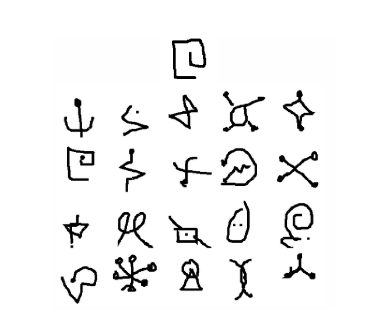
\includegraphics[height=.5\textheight]{oneshotnway}
                \end{centering}
        \end{enumerate}
    \end{block}
    \begin{block}{MAML}
        \begin{enumerate}
            \item Previous approaches to few-shot learning are usually specific to certain problems or model architecture
            \item This paper proposed a meta-learning algorithm (MAML) that is
                \begin{enumerate}
                    \item general to different problem - supervised learning, reinforcement learning
                    \item agnostic to different model architectures - CNN, RNN
                \end{enumerate}
        \end{enumerate}
    \end{block}

\end{frame}

\begin{frame}[t]{MAML In a Nutshell}
    \begin{center}
        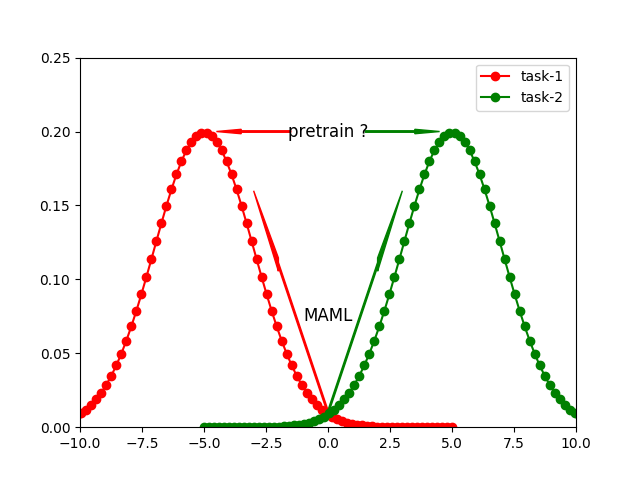
\includegraphics[height=.5\textheight,width=.8\textwidth]{nutshell}
    \end{center}
    \begin{enumerate}
        \item MAML searches for a point maximizing improvement of k-step fine-tuning for all tasks
        \item Pre-training searches for a point maximizing performance on pre-training dataset
    \end{enumerate}
\end{frame}

\section{Formulation}
\begin{frame}[t]{Notations}
    \begin{block}{A formal \& general definition of Model and Task}
        \begin{enumerate}
            \item Model: $f: \mathcal{X}\rightarrow \mathcal{A}$
            \item Task: $\mathcal{T}=\{H,\mathcal{L}(x_1,a_1,\cdots,x_H,a_H),q(x_1),q(x_{t+1}|x_t,a_t)\}$
                \begin{enumerate}
                    \item Episode Length: $H$
                    \item Loss function: $\mathcal{L}: \mathcal{X}^\mathcal{H}\times\mathcal{A}^{H}\rightarrow \mathcal{R}$
                    \item Initial observation distribution: $q(x_1)$
                    \item Transition distribution: $q(x_{t+1}|x_t,a_t)$
                \end{enumerate}
        \end{enumerate}
    \end{block}

    \begin{block}{Examples}
        \begin{center}
            \begin{tabular}{cll}
                \hline
                              & Supervise Learning        & Reinforcement Learning \\ \hline
                $\mathcal{X}$ & images                    & states                 \\ \hline
                $\mathcal{A}$ & classification            & action                 \\ \hline
                $H$           & 1                         & arbitrary              \\ \hline
                $\mathcal{L}$ & categorical cross-entropy & negative reward        \\ \hline
            \end{tabular}
        \end{center}
    \end{block}
\end{frame}

\begin{frame}[allowframebreaks]{Meta-Learning Algorithm}
    \begin{enumerate}
        \item The meta-learner maintain the model parameter $\theta$
        \item The task searcher perform SGD to find better $\theta\rightarrow\theta'_i$ on each task $\mathcal{T}_i$
        \item Update $\theta$ according to the \textbf{loss on $\theta'_i$} summing over all taks
            \begin{center}
                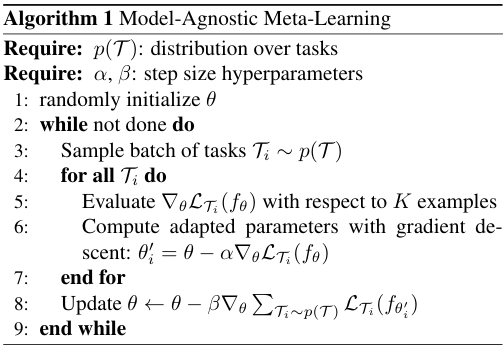
\includegraphics[height=.6\textheight]{alg1}
            \end{center}
    \end{enumerate}

    \begin{enumerate}
        \item The task searching update $\theta'_i=\theta-\alpha\nabla_{\theta}\mathcal{L}_{\mathcal{T}_i}(f_{\theta})$ can easily be generalized to $K$ updates with $K$ samples per task.
        \item MAML doesn't overfit easily because the meta-learner's update $\theta$ on loss $\mathcal{L}_{\mathcal{T}_i}(f_{\theta'_i})$ instead of $\mathcal{L}_{\mathcal{T}_i}(f_{\theta})$
        \item This makes that even one sample for each task enough
    \end{enumerate}

    \begin{block}{Computation Expense}
        Note that in meta-learner's update (using $\theta$ in place of $f_{\theta}$)
        \begin{align*}
             & \nabla_{\theta}\mathcal{L}_{\mathcal{T}_i}(\theta'_i) & \\
            = &  \nabla_{\theta} \theta'_i \nabla_{\theta'} \mathcal{L}_{\mathcal{T}_i}(\theta'_i) & \text{(chain rule)} \\
            = & \nabla_{\theta} \left[\theta-\alpha\nabla_{\theta}\mathcal{L}_{\mathcal{T}_i}(\theta)\right] \nabla_{\theta'} \mathcal{L}_{\mathcal{T}_i}(\theta'_i)  & \text{(task update)}\\
            = & \left[ I -\alpha\nabla^2_{\theta}\mathcal{L}_{\mathcal{T}_i}(\theta)) \right] \nabla_{\theta'} \mathcal{L}_{\mathcal{T}_i}(\theta'_i) &
        \end{align*}
        we need to calculate the hessian-vector product $\nabla^2 \mathcal{L}_{\mathcal{T}_i}(\theta)\nabla_{\theta'} \mathcal{L}_{\mathcal{T}_i}(\theta'_i)$, when omitted, $\nabla_{\theta'} \mathcal{L}_{\mathcal{T}_i}(\theta'_i)$ is the first order approximation to the meta-learner's gradient $\nabla_{\theta}\mathcal{L}_{\mathcal{T}_i}(\theta'_i)$.
    \end{block}

    \begin{enumerate}
        \item Algorithm 1 can be adapted to different tasks including supervised learning \& reinforcement learning by choosing different task loss function $\mathcal{L}_{\mathcal{T}_i}$ and data sample procedure
        \item For example, in reinforcement learning:
            \begin{enumerate}
                \item The model $f_{\phi}$ is a policy network that maps from states $x_t\in \mathcal{X}$ to a distribution over actions $a_t\in\mathcal{A}$ at each time step $t\in\{1,\cdots,H\}$.
                \item Given the initial state $x_0$, the model samples a trajectory $(x_0,a_0,x_1,a_1,\cdots,x_H)$. In K-shot reinforcement learning, the model is limited to sample only $K$ trajectories.
                \item The loss function is the negative expectation of the total reward
                    \begin{equation*}
                        \mathcal{L}_{\mathcal{T}_i}(f_{\phi}) = -\mathbb{E}_{x_t,a_t\sim f_{\phi},q_{\mathcal{T}_i}} \left[ \sum_{i=1}^H R_i(x_t,a_t) \right]
                    \end{equation*}
            \end{enumerate}
            \scriptsize{* This loss is generally not differentiable w.r.t. $\phi$. For more information, please check this \href{https://lilianweng.github.io/lil-log/2018/04/08/policy-gradient-algorithms.html}{blog post} and this \href{http://ipod825.github.io/presentations/variational_approaches_for_autoencoding_generative_adversarial_networks/main.pdf}{slide}}
    \end{enumerate}
    \framebreak
    \begin{enumerate}
        \item Algorithm 1 can then be adapted as Algorithm 3
        \item Note that we sample from $\mathcal{T}_i$ two times for task update (using current $\theta$) and meta-learner update (using $\theta_i$).
    \end{enumerate}
    \begin{center}
        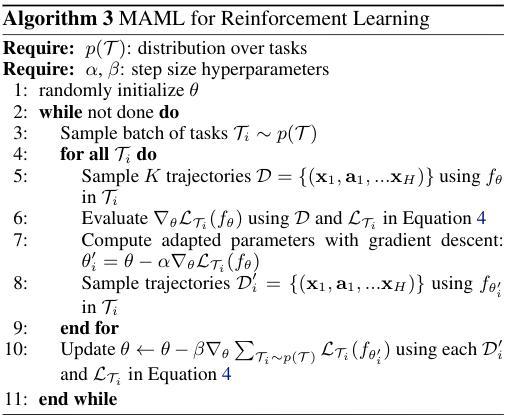
\includegraphics[height=.6\textheight]{reinforcement}
    \end{center}
\end{frame}

\section{Evaluation}
\begin{frame}[t]{Sinusoid Regression}
    \begin{enumerate}
        \item Sin functions with different amplitude ranging $[0.1,5.0]$
        \item Each task (sin functions) has $K=10$ samples
        \item The task searcher adopt single step
    \end{enumerate}
    \begin{center}
        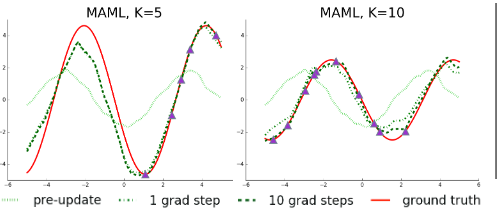
\includegraphics[height=.3\textheight,width=\textwidth]{sinexp1}
        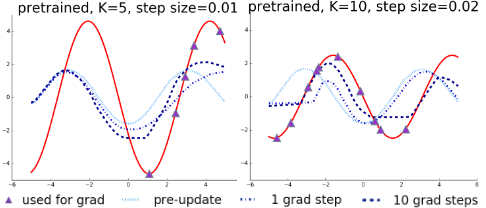
\includegraphics[height=.3\textheight,width=\textwidth]{sinexp2}
    \end{center}
\end{frame}

\begin{frame}{Classification}
    \begin{enumerate}
        \item 5-way, K-shot image classification on MiniImagenet
        \item Siamese nets, matching nets, and the memory module approaches are all specific to classification, and are not directly applicable to regression or RL scenarios.
    \end{enumerate}
    \begin{center}
        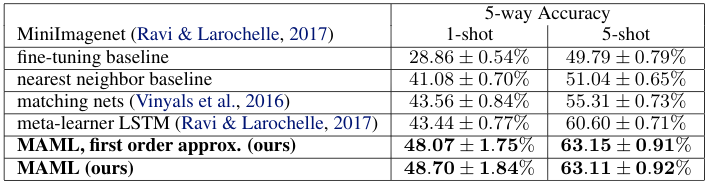
\includegraphics[height=.5\textheight,width=\textwidth]{classificationexp}
    \end{center}
\end{frame}

\begin{frame}[t]{Matching Net}
    \begin{center}
        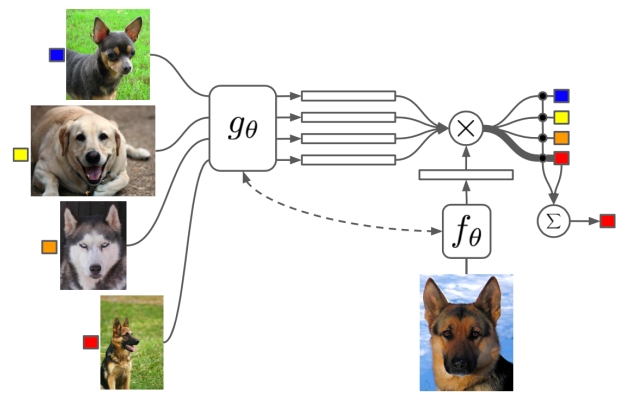
\includegraphics[height=.7\textheight]{matchingnet}
    \end{center}
\end{frame}

\begin{frame}[t]{Reinforcement Learning}
    \begin{enumerate}
        \item Locomotion: agent needs to learn to run in a particular direction or at a particular velocity.
        \item Each task means running in different directions or velocities.
    \end{enumerate}
    \begin{center}
        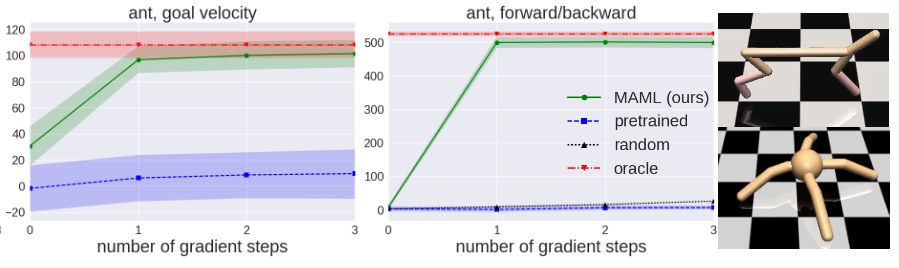
\includegraphics[height=.4\textheight,width=\textwidth]{reinforceexp}
    \end{center}

\end{frame}



% \bibliographystyle{apalike}
% \bibliography{main}

\end{document}
